% Hinh: paper/paper1_qmi/figs_revision/fig9 (make_paper1_figures.py --qmi). Caption viet lai cho QMI.
\begin{figure}[t]
  \centering
  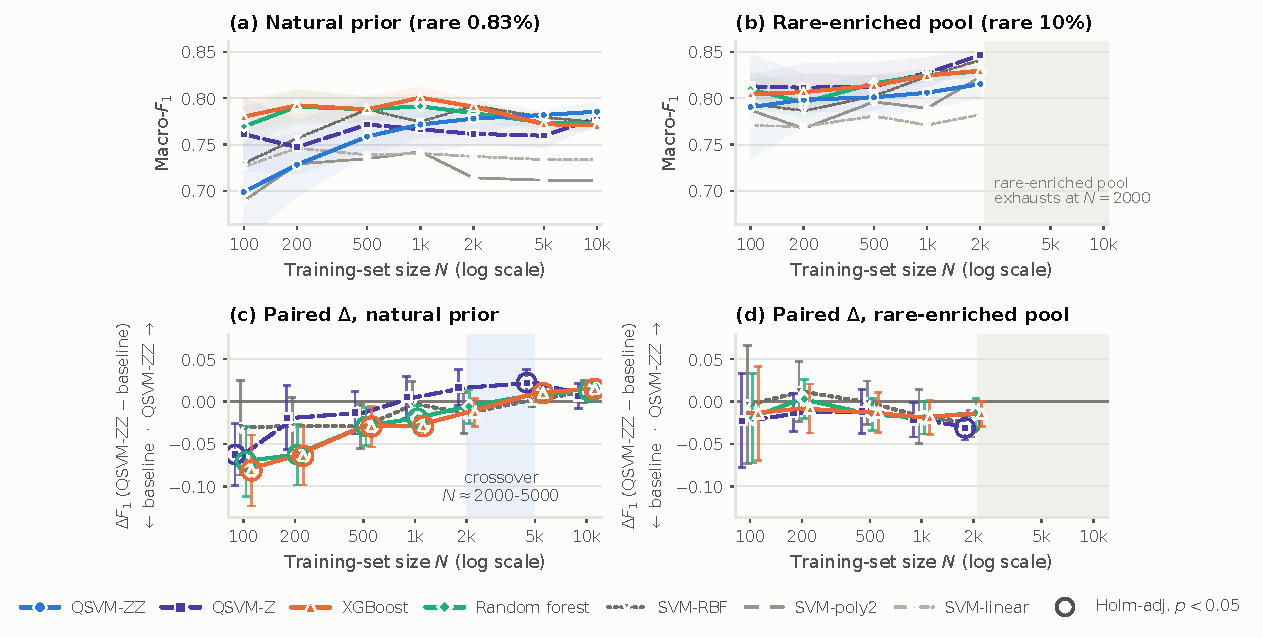
\includegraphics[width=\textwidth]{figs_revision/fig9_learning_curve_nslkdd.pdf}
  \caption{Training-set size on NSL-KDD, scored on the full KDDTest$^+$ set. (a,~b) Mean
    macro-$F_1$ over ten runs with $95\%$ bands under the natural prior (a) and the rare-enriched
    pool (b). (c,~d) Paired differences \QSVM{} minus each baseline, circled where the
    Holm-adjusted $p<0.05$. The enriched pool cannot be sampled beyond $N=2000$ without runs
    sharing rare records, so panels (b) and (d) end one step before the interval in which the
    sign changes under the natural prior.}
  \label{fig:learning-curve}
\end{figure}
